\documentclass[fleqn,numbers=noenddot,headinclude,%twoside,%1headlines,%
				11pt,a4paper,footinclude,%
				cleardoublepage=empty,abstractoff %
                ]{scrartcl}

\usepackage[hyphens]{url}
\usepackage{float}

\def\tomas{Tom\'{a}\v{s} Peterka}
\def\tomasid{peterto8}
\def\franta{Franti\v{s}ek Hejl}
\def\frantaid{hejl}
\def\jan{J\'{a}n Tka\v{c}\'{i}k}
\def\janid{tkacijan}
\def\frantaid{hejl}

\def\laboratoryname{Ov\v{e}\v{r}en\'{i} metody CTEX}
\def\date{\today}


\usepackage[automark]{scrpage2}



\usepackage{makerobust}

%\DeclareRobustCommand{\graffito}[1]{\marginpar{%
%    \slshape\footnotesize%\small%
%    %\ifodd\thepage\raggedright\else\raggedleft\fi%
%    \raggedright
%    \parindent=0pt\lineskip=0pt\lineskiplimit=0pt\baselineskip=11pt
%    \tolerance=2000\hyphenpenalty=300\exhyphenpenalty=300%
%    \doublehyphendemerits=100000\finalhyphendemerits=\doublehyphendemerits%
%    %\raggedright%
%    \hspace{0pt}#1}}

\usepackage[
		%textwidth=15cm,
	    top=4cm,
	    bottom=4cm,
	    left=3.5cm,
	    right=3cm,
%	    includeheadfoot,
%	    showframe,
	    footskip=1cm,
	    marginparwidth=1.9cm,
%	    textheight=22cm
		]{geometry}

\usepackage[czech]{babel}
\usepackage[T1]{fontenc}
\usepackage[utf8]{inputenc}
\usepackage{abstract}

%\usepackage{courier}

\usepackage{graphicx}

\usepackage{marvosym}
%\usepackage{array}
%\usepackage{booktabs}

\usepackage[table]{xcolor}
\definecolor{codeback}{gray}{.5}
\definecolor{darkblue}{rgb}{0,0,.5}

\usepackage{listings}
%\usepackage{listingsutf8}
\lstdefinestyle{java}{
      language=java,
      identifierstyle=\ttfamily,
      keywordstyle=\bfseries\ttfamily\color[rgb]{0,0,1},
      commentstyle=\color[rgb]{0.133,0.545,0.133},
      stringstyle=\color[rgb]{0,0,1},
      numbers=left,
      numbersep=7pt,
      numberstyle=\sffamily\tiny,
      basicstyle=\ttfamily\small,
      aboveskip={.3\baselineskip},
      %columns=fullflexible,
      showstringspaces=false,
      breaklines=true,
      tabsize=2,
      showspaces=false,
      frame=leftline,
      backgroundcolor=\color{white},
      rulesepcolor=\color{red}
}

\usepackage{framed}
%\usepackage{pstricks}
\usepackage{tikz}
\usetikzlibrary{shapes}
\usetikzlibrary{arrows}
\usetikzlibrary{calc}


\usepackage{calc}
\usepackage{amsmath}
\usepackage{amssymb}
\usepackage{nccmath}
%\usepackage{dsfont}
\usepackage{empheq}
\usepackage[normalem]{ulem}
\newcommand{\msout}[1]{\text{\sout{\ensuremath{#1}}}}
%\usepackage{lmodern}

\setlength{\mathindent}{1ex}

\usepackage{float}


\usepackage{textcomp} %Paket mit Sonderzeichen, Symbolen 
%\usepackage{pifont}% zapfdingbats für besondere Zeichen
\usepackage{eurosym} %schönes Eurozeichen mit \euro auch der Schrift angepaßt
\usepackage{eco}
\usepackage[osf, sc]{mathpazo}
\linespread{1.03}

\usepackage{microtype}
\usepackage[scaled=0.85]{beramono}

%\usepackage[euler-digits]{eulervm}
%\usepackage{fouriernc}

\usepackage[framed]{ntheorem}
\usepackage{footnote}

\usepackage{float}
\usepackage{dblfloatfix}

%\usepackage{cpation}

%\usepackage{multicol}


\PassOptionsToPackage{hyphens}{url}\usepackage[pdftex,breaklinks]{hyperref}


%\usepackage{breakurl}
\hypersetup{%
    colorlinks=true, linktocpage=false, pdfstartpage=1, pdfstartview=FitV,%
    % uncomment the following line if you want to have black links (e.g., for printing)
    colorlinks=false, 
    linktocpage=false, pdfborder={0 0 0}, pdfstartpage=1, pdfstartview=FitV,% 
    breaklinks=true, pdfpagemode=UseNone, pageanchor=true, pdfpagemode=UseOutlines,%
    plainpages=false, bookmarksnumbered, bookmarksopen=true, bookmarksopenlevel=3,%
    hypertexnames=true, pdfhighlight=/O,%hyperfootnotes=true,%nesting=true,%frenchlinks,%
    urlcolor=webbrown, linkcolor=darkblue, citecolor=webgreen, %pagecolor=RoyalBlue,%
    %urlcolor=Black, linkcolor=Black, citecolor=Black, %pagecolor=Black,%
    %pdftitle={\myTitle},%
    %pdfauthor={\textcopyright\ \myName, \myUni, \myFaculty},%
    pdfsubject={},%
    pdfkeywords={},%
    pdfcreator={pdfLaTeX},%
    pdfproducer={LaTeX}%
}





\newcounter{ale}

\pagestyle{scrheadings}
\clearscrheadfoot
\ofoot{Lab \laboratorynr{} -- \laboratoryname}
\ifoot{\tomas{} \& \franta}
\ihead{\leftmark}
\ohead{\pagemark}


\setheadsepline{0.4pt}
\setfootsepline{0.4pt}


\definecolor{lightgray}{rgb}{.9,.9,.9}
\definecolor{lightblue}{HTML}{CCCCFF}




\clubpenalty = 10000
\widowpenalty = 10000
\displaywidowpenalty = 10000

%\usepackage[subfigure]{tocloft}
%\renewcommand{\cftpartleader}{\cftdotfill{\cftdotsep}} % for parts
%\renewcommand{\cftchapleader}{\cftdotfill{\cftdotsep}} % for chapters
%\renewcommand{\cftsecleader}{\cftdotfill{\cftdotsep}} % for sections

\usepackage[sl,SF]{subfigure}
\usepackage{wrapfig}
\usepackage[hang,marginal]{footmisc}
\usepackage[justification=raggedright, margin=1cm,singlelinecheck=false,format=hang, labelfont={sl,small,rm},font={small,sf}, skip=10pt]{caption}
\renewcommand*\thesubfigure{\alph{subfigure}}

\DeclareMathOperator*{\argmax}{arg\,max}
\DeclareMathOperator*{\abs}{abs}

\makeatletter
\newcommand\wrapfill{\par
    \ifx\parshape\WF@fudgeparshape
    \nobreak
    \vskip-\baselineskip
    \vskip\c@WF@wrappedlines\baselineskip
    \allowbreak
    \WFclear
    \fi
}
\makeatother

\setlength{\intextsep}{6pt}

\usepackage{titlesec}
\titleformat{\section}{\large\bfseries}{\thesection}{1em}{}
\titleformat{\subsection}{\normalsize\bfseries}{\thesection}{1em}{}
\titleformat{\subsubsection}{\normalsize\bfseries}{\thesection}{1em}{}

\usepackage{amsmath}
\usepackage{graphicx}

\begin{document}

\makesavenoteenv[figure*]{figure}
\pagestyle{empty}
\onecolumn
%%Manuelle titelseite
\null  % Empty line
\nointerlineskip  % No skip for prev line
\vspace*{-1cm}
\begin{center}


\includegraphics[width=7cm,keepaspectratio=true]{./imgs/fit_logo.pdf}\\[0.3cm]
Czech Technical University\\
Faculty of Informatics

\vspace{1.2cm}

\Large MI-ROZ -- Rozpoznávání\\[0.5cm]
\laboratoryname \normalsize\\

\vspace{0.7cm}

\begin{tabular}{ccc}
\tomas & \franta & \jan \\
\tomasid @fit.cvut.cz & \frantaid @fit.cvut.cz & \janid @fit.cvut.cz \\
\end{tabular} \\[0.7cm]
\date
\end{center}
\vfill
\begin{abstract}
Práce popisuje implementaci algoritmu CTEX a jeho otestování na sérii zkušebních dat z ÚTIA (Ústav teorie informace a automatizace AV ČR).
\end{abstract}
\vfill
\tableofcontents

\clearpage

\pagestyle{scrheadings}
\setcounter{page}{1}

\section{Implementace CTex algoritmu}
\subsection{GB-FAB filter}
\label{sub:gb-fab}
Anisotropický filter pro zvýraznění středně silných hran. Implementace podle zadání nebyla problém a nevznikly žádné odchylky. Jedině snad, že gradient je počítán 4 směrově, místo 8 směrově. V článku není jasně definováno jak přesně gradient počítali.
Tento filter používá upravenou hodnotu gradientu (pomocí mediánu z gradientu ve všech osách). Rozpuštění okolních pixelů do středového je řízena funkcí s průběhem na obrázku \ref{img:gbfab} a proto filter zvýrazňuje střední hrany, ponechává hrany ostré a zbytek celkem agresivně rozpouští do okolí.
\begin{figure}[htp]
\centering
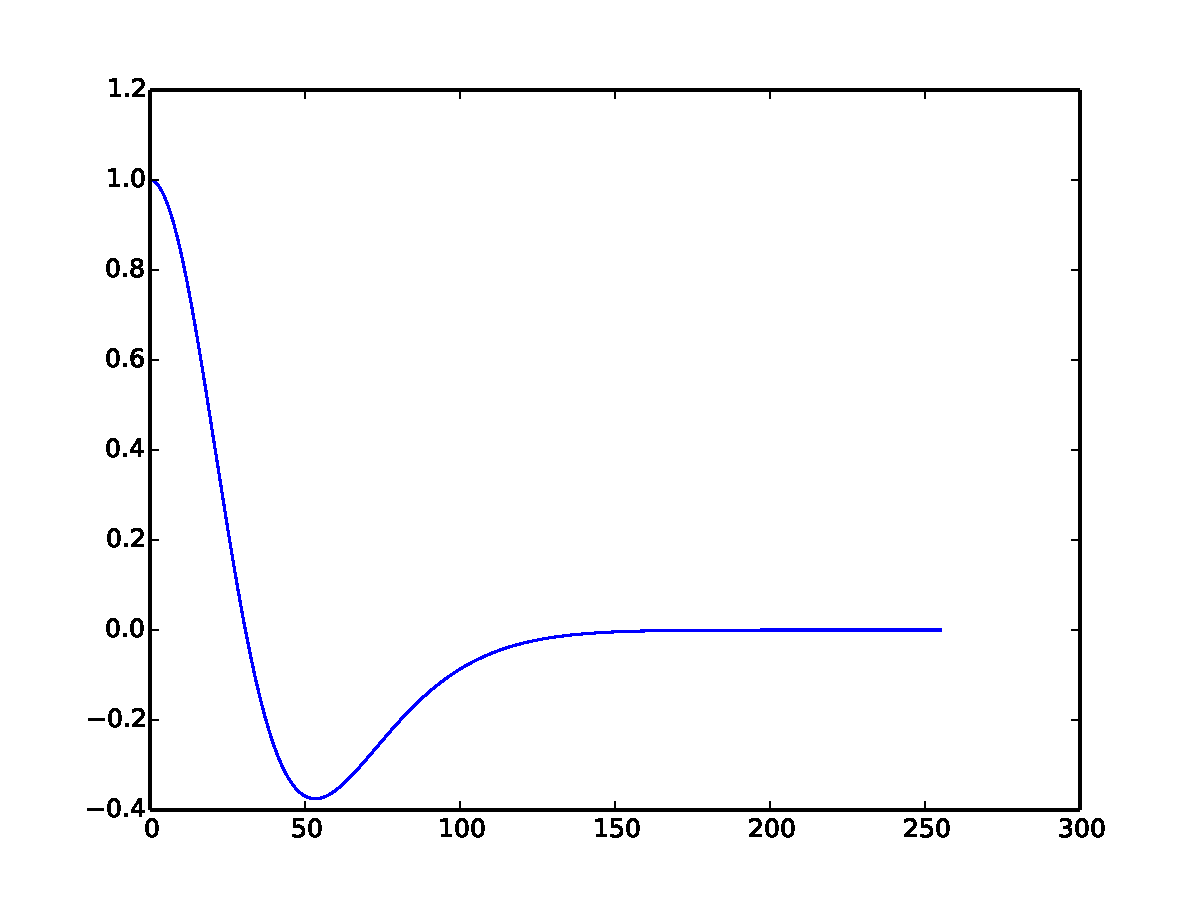
\includegraphics[width=\textwidth]{plots/dfab_function.pdf}
\caption{Funkce rozpuštění gradientu do středu}
\label{img:gbfab}
\end{figure}
% subsection  (end)

\subsection{Výběr ideálního počtu shluků}
\label{sub:som}
Tato procedura sestává z více kroků. Nejdříve se pomocí SOM určí nejlepší počet centroidů a ty se poté předají do k-means algoritmu.

\subsubsection{Výběr dominantních barev} Slouží k iniciaci SOM mapy o velikosti 16 (čtverec $4\times4$), aby se nepoužívaly náhodné hodnoty. Prvník krokem je redukce barevného prostoru z (255, 255, 255) do (8, 8, 8) a zde sestrojíme 3D histogram. Z tohoto histogramu sebereme 16 barev s nejvyšší hodnotou pro iniciaci SOM mapy.
%subsubsection  (end)

\subsubsection{SOM analýza}
Po provedení a ukončení iterativního SOM algoritmu spočítáme váhy pro každý neuron v síti a spojujeme takové, které mají vzdálenost vah $<0.3$. Pokaždé když spojujeme 2 shluky, vybíráme jako reprezentanta ten s menší \textit{confidence} (vnitřní rozptyl částic). Výsledný počet neuronů/shluků je výstupem této části.
%subsubsection  (end)
% subsection  (end)

\subsection{Shlukování obrázků}
\label{sub:kmeans}

% subsection  (end)

\subsection{Multispace K-means}
\label{sub:multi-kmeans}
lorem ipsum
% subsection  (end)

\subsection{Extrakce textur}
\label{sub:textury}
lorem ipsum
% subsection  (end)

\subsection{ASKM}
\label{sub:askm}
lorem ipsum
% subsection  (end)


\section{Vyhodnocení}
\label{sec:vyhodnoceni}
lorem ipsum
% section  (end)

\section{Závěr}
\label{sec:zaver}
lorem ipsum
% section  (end)
%\lstset{style=java}
%\begin{lstlisting}
%
%\end{lstlisting}

\end{document}
